% ------------------------------------------------------------------------------
% 4. JUSTIFICACIÓN
% ------------------------------------------------------------------------------
\subsection{4. Justificación}\label{sec:justificacion}
% [INSTRUCCIÓN]: Justificar la pertinencia del proyecto desde las dimensiones
% técnica, social, económica y académica.

El desarrollo del Sistema de Información Web y Móvil para la Gestión Integral del Comedor Universitario de la UAGRM se justifica desde tres dimensiones fundamentales: la operativa y técnica, la social y la económica.

\subsubsection{4.1. Justificación operativa y técnica}\label{sec:justificacion_operativa_tecnica}

La capacidad administrativa actual presenta una severa limitación, ya que únicamente se logra revisar un aproximado de 8,000 carpetas físicas por gestión. La implementación de un modelo de inteligencia artificial para la preselección automatizada permitirá procesar y evaluar el 100\% de las 20,000 solicitudes recibidas anualmente. Con ello se elimina el cuello de botella operativo y se agilizan los tiempos de respuesta de la DUBSS, de modo que el personal administrativo pueda enfocar sus esfuerzos de auditoría exclusivamente en los expedientes que el sistema señale con el mayor puntaje de prioridad (véase la Figura~\ref{fig:cuello_botella}).

\begin{figure}[htbp]
\caption{Brecha entre las solicitudes recibidas, las carpetas revisadas y las becas adjudicadas en el proceso manual de gestión}
\label{fig:cuello_botella}
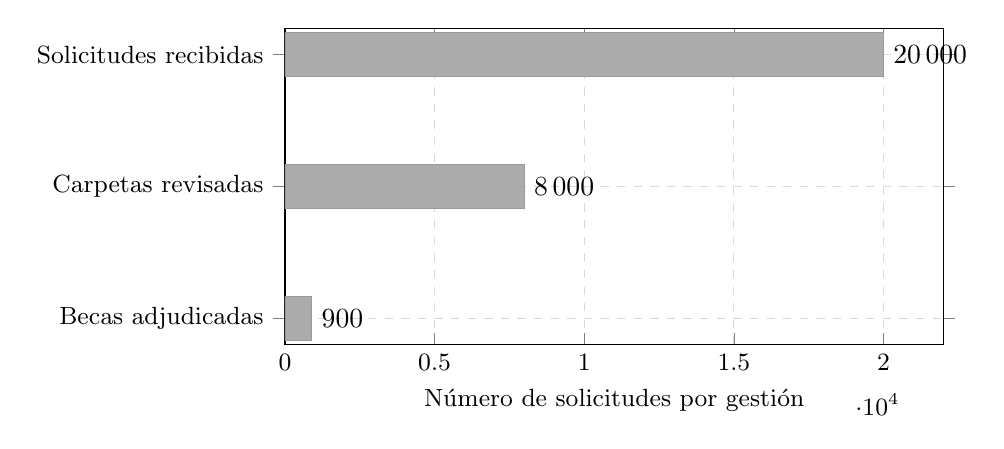
\begin{tikzpicture}
\begin{axis}[
    xbar,
    width=0.82\linewidth,
    height=5.6cm,
    bar width=16pt,
    xmin=0, xmax=22000,
    xtick={0,5000,10000,15000,20000},
    xticklabel={\pgfmathprintnumber{\tick}},
    xlabel={Número de solicitudes por gestión},
    ytick={1,2,3},
    yticklabels={Becas adjudicadas, Carpetas revisadas, Solicitudes recibidas},
    nodes near coords,
    nodes near coords align={horizontal},
    nodes near coords style={/pgf/number format/1000 sep={\,}},
    grid=major,
    grid style={dashed, gray!30},
    tick label style={font=\small},
    label style={font=\small},
]
\addplot[
    fill=gray!65,
    draw=gray!80,
] coordinates {
    (900,   1)
    (8000,  2)
    (20000, 3)
};
\end{axis}
\end{tikzpicture}

\smallskip
\noindent\textit{Nota.} Elaboración propia en base a los datos institucionales de la DUBSS. De las 20,000 solicitudes recibidas en cada gestión, aproximadamente 8,000 carpetas logran revisarse, mientras que únicamente cerca de 900 cupos resultan efectivamente adjudicados.
\end{figure}

\subsubsection{4.2. Justificación social}\label{sec:justificacion_social}

El proceso de evaluación manual vigente genera una exclusión involuntaria, pues alrededor del 60\% de los postulantes (cerca de 12,000 estudiantes) no llega a ser evaluado. El algoritmo de priorización socioeconómica resolverá esta brecha de equidad al garantizar que los cerca de 900 cupos disponibles para la beca comedor se asignen de manera transparente, medible y justa a los estudiantes que presenten el mayor nivel de vulnerabilidad, erradicando los sesgos propios del método de revisión al azar o por orden de llegada. La Tabla~\ref{tab:necesidad_sistema} contrasta la situación actual con la esperada tras la implantación del sistema.

\begin{table}[htbp]
\caption{Comparativa del proceso de asignación de la beca comedor: situación actual frente a la esperada con el sistema propuesto}
\label{tab:necesidad_sistema}
\begin{threeparttable}
\begin{tabular}{lc c}
\toprule
Indicador & Proceso manual actual & Con el sistema propuesto \\
\midrule
Solicitudes evaluadas por gestión & 8,000 (40\%) & 20,000 (100\%) \\
Postulantes sin evaluación & 12,000 (60\%) & 0 \\
Cupos disponibles & 900 & 900 \\
Criterio de selección & Azar u orden de llegada & Priorización socioeconómica \\
Transparencia y trazabilidad & Baja & Alta \\
\bottomrule
\end{tabular}
\begin{tablenotes}
\item \textit{Nota.} Elaboración propia en base a los datos institucionales de la DUBSS. Las cifras corresponden a una gestión académica ordinaria y pueden variar según el presupuesto asignado.
\end{tablenotes}
\end{threeparttable}
\end{table}

\subsubsection{4.3. Justificación económica y operativa: optimización de recursos}\label{sec:justificacion_economica}

Aunque el proceso final exige la validación física de los respaldos, el sistema actuará como un embudo digital que reduce drásticamente el volumen de recepción documental. En lugar de exigir, recepcionar y almacenar administrativamente 20,000 carpetas físicas al inicio de cada gestión, la DUBSS solicitará la documentación en físico únicamente a las carpetas con los puntajes de precalificación más altos. Esto transforma un proceso logísticamente insostenible en uno altamente eficiente, generando un ahorro significativo en horas-hombre y espacio de archivo para la universidad y evitando gastos de impresión y tramitación en vano para la inmensa mayoría de los estudiantes que no llegarán a la fase final de selección. La Tabla~\ref{tab:proyeccion_recepcion} proyecta la recepción documental actual y la estimada con el sistema de preselección.

\begin{table}[htbp]
\caption{Proyección de la recepción y gestión documental: proceso actual frente al esquema de preselección automática}
\label{tab:proyeccion_recepcion}
\begin{threeparttable}
\begin{tabular}{lc c}
\toprule
Aspecto & Proceso manual actual & Con preselección automática \\
\midrule
Carpetas solicitadas en físico & 20,000 & Aprox. 2,700 (finalistas) \\
Carpetas almacenadas & 20,000 & Aprox. 2,700 \\
Hojas de papel gestionadas & Alto & Mínimo \\
Horas-hombre de revisión & Elevadas & Enfocadas y auditadas \\
Trámite de impresión en vano & Mayoría de postulantes & Solo fase final \\
\bottomrule
\end{tabular}
\begin{tablenotes}
\item \textit{Nota.} Elaboración propia. La proyección de 2,700 carpetas se basa en un margen de revisión equivalente a tres carpetas por cada uno de los 900 cupos disponibles, a fin de cubrir desistimientos o inconsistencias documentales.
\end{tablenotes}
\end{threeparttable}
\end{table}